\chapter{Experimental setup}\label{sec:experimental_setup}

This chapter delineates the covariate shift setting within the 
supervised classification framework and introduces an operative
formulation of posterior agreement. This formulation enables
robustness-based model selection in discrete hypothesis class scenarios.

% This formulation represents 
% the cornerstone of this work as it enables robustness-based
% model selection in discrete hypothesis class problems.

\section{Problem formulation}

Out of all the possible learning problems in which a distribution shift
can be defined, this project will focus on the supervised classification
of images. The function space to navigate is composed of parametrized
classifiers.

\begin{definition}[\emph{Classifier}]\label{def:classifier}
    Let $\mathcal{X}$ and $\mathcal{Y} \subset\mathbb{N}$ be the input and output spaces of the target function, respectively.
    Let $K \in \mathbb{N} < \infty$ be the cardinality of $\mathcal{Y}$.

    \begin{itemize}
        \item Let $\Phi$ be a feature extractor, mapping the input space to a $d$-dimensional feature space.
            $$ 
            \begin{aligned}
                \Phi: \mathcal{X} & \longmapsto \mathbb{R}^d \\
                x & \longmapsto \Phi(x) = z
            \end{aligned}
            $$

        \item Let $\bm{F}$ be a discriminant function, assigning a score
        to each of the $K$ classes. 
            $$
            \begin{aligned}
                \bm{F}: \mathbb{R}^d  & \longmapsto \mathbb{R}^K \\
                z & \longmapsto \left ( F_1(z), \dots, F_K(z) \right ) = \bm{F}(z)
            \end{aligned}
            $$
        \item Let $\eta$ be a decision rule, yielding the class label from a vector of scores.
        It will be set to the maximum a posteriori (MAP) rule.
            $$
                \begin{aligned}
                    \eta: \mathbb{R}^K & \longmapsto \mathcal{Y} = \{1, \dots, K \} \\
                    \bm{F}(z) & \longmapsto \hat{y} = \arg \max_{k} F_k(z)
                \end{aligned}
            $$
    \end{itemize}

    A $K$-class classifier can be defined as the composition of these three functions:
    $$
    c = \eta \circ \bm{F} \circ \Phi.
    $$

    The results presented in this work are limited to neural network classifiers, which
    entail a parametrization in $\Gamma \subseteq \mathbb{R}^{|\Gamma|}$ that can be expressed
    as

    $$
        \begin{aligned}
        c: \mathcal{X} \times \Gamma & \longmapsto \mathcal{Y} = \{1, \dots, K \} \\
        (x, \gamma) & \longmapsto c(x; \gamma) = \hat{y},
        \end{aligned}
    $$

    thus $c(x; \gamma) = \eta \circ (\bm{F} \circ \Phi)(x; \gamma)$. \\
\end{definition}

The concepts introduced in the previous chapter provide the 
foundation for the formalization of the learning problem in which our 
robustness experiments will be conduted. We will refer to this 
problem as a $K$-class classification.

\begin{definition}[\emph{$K$-class classification}]
    Let $D \in \mathcal{D}$ be a supervised dataset.
    Let $c$ be a neural network classifier, parametrized
    in $\Gamma \subseteq \mathbb{R}^{|\Gamma|}$.
    Let $\operatorname{RRM}$ be the regularized risk minimization problem for $c$ on $D$.
    Let $L$ be the cross-entropy loss function for classifier $c$, computed as

    $$
    L(x, y) = - \log F_y(\Phi(x); \gamma).
    $$

    The $K$-class classification is the $\operatorname{RRM}$ problem parametrized in $\Gamma$
    with cross-entropy loss $L$:
    $$
        \gamma^* = \arg \min_{\gamma \in \Gamma} - \frac{1}{N}\sum_{n=1}^{N} \log F_{y_n}(x_n; \gamma) + \lambda \Omega(\gamma)
    $$

\end{definition}

No further characterization of the regularization factor $\lambda \Omega(\gamma)$ will be provided
in this section, as the specific learning algorithms considered will be introduced
later in the text.

\section{Robustness in covariate shift settings}\label{sec:robustness_to_covariate_shift}

The concept of robustness, as defined in the previous chapter, entails
a measure of the stability of the learner to the randomness of
the data sampling process, but also requires an adequate characterization
of such randomness. In the context of the $K$-class classification
problem, sampling randomness can be formalized as a shift in the
distribution of the input space, also known as covariate shift. 

\begin{definition}[\emph{Covariate shift}]
    Let $\bm{x}'$ and $\bm{x}''$ be two samples of $\bm{X} \overset{\text{iid}}{\sim} X$ with size $N$.
    A covariate shift exists between $\bm{x}'$ and $\bm{x}''$ if their
    (empirical) distributions are significantly different\footnote{
        The notion of difference relies on the nature of the data. Common measures 
        include statistical distances such as the Kullback-Leibler divergence, 
        Wasserstein distance, or even simpler metrics like the difference in 
        means or variances. These methods help establish whether observed 
        differences are statistically significant. \cite{quinonero-candelaDatasetShiftMachine2009}
    }
    for $N$ large enough. This is expressed as:

    $$
    \mathbf{P}_{\bm{x}'} \not \sim \mathbf{P}_{\bm{x}''}.
    $$
    
    It must be noted that, since the target function is assumed
    to be invariant (see Section \ref{sec:intro_ood}), 
    the true distribution over the output space
    remains the same \cite{quinonero-candelaDatasetShiftMachine2009}.
\end{definition}

The presence of covariate shift as defined above already leads
to a non-zero generalization error, given that $\bm{x}'$ and $\bm{x}''$ 
represent different randomness instantiations and result in different 
learning outcomes. Nevertheless, this definition can be further
expanded to encompass more practical sources of shift in the 
context of classification tasks.

\begin{definition}[\emph{Distribution shift}]\label{def:domain_shift}
    Let $X'$ and $X''$ be two random variables associated to different sampling 
    experiments in $\mathcal{X}$ such that $P_{X'} \not \sim P_{X''}$.
    The effective randomness entailed by their respective measurement
    process is also different in general (i.e. $\mathcal{T}_{\mathbf{X}'} \neq \mathcal{T}_{\mathbf{X}''}$).
    In such case

    $$
        \bm{x}' \sim \bm{X}' \overset{\text{iid}}{\sim} X' \text{ and } \bm{x}'' \sim \bm{X}'' \overset{\text{iid}}{\sim} X''
    $$

    lead to a covariate shift known as out-of-distribution, given that 
    the fundamental source of variability is the difference in the probability
    measure over the support induced by each experiment
    \cite{quinonero-candelaDatasetShiftMachine2009}.
    In simpler terms, $X' \neq X'' \Longrightarrow \mathbf{P}_{\bm{x}'} \not \sim \mathbf{P}_{\bm{x}''}$ in general.
\end{definition}

In the out-of-distribution setting, $\bm{x}'$ and $\bm{x}''$ are
drawn from different random variables, each with a distinct probability 
landscape over the support, namely source and target domains, that result 
in implicit and/or explicit differences (sometimes unbalanced) in the distribution of some features.
Therefore, empirical distributions $\mathbf{P}_{\bm{x}'}$ and $\mathbf{P}_{\bm{x}''}$ will
be different in general and induce a covariate shift that leads
to a non-zero generalization error.

\begin{definition}[\emph{Adversarial shift}]
    Let $\bm{x}' \sim \bm{X}$ be a sample drawn from experiment
    $X$. Let $\bm{\Delta}$ be a perturbation over
    the sample space. In this case, $\bm{x}''$ is generated by perturbing $\bm{x}'$ as

    $$
    \bm{x}'' = \bm{x}' + \bm{\Delta},
    $$

    which induces a covariate shift known as adversarial, given that
    perturbation $\bm{\Delta}$ is crafted ad-hoc to hinder the 
    output of the model.
\end{definition}

In the adversarial setting, sampling randomness is not the source of
covariate shift, as both $\bm{x}'$ and $\bm{x}''$ arise from
the same realization of the experiment. \\

Overall, this work must pursue a wider approach to generalization  
that does not only comprise the implicit
randomness embedded in each realization $\bm{x} \sim \bm{X}$
but also the explicit shift in the distribution of the input space
generated by intentional or unintentional perturbations of the 
data generation process. This broader interpretation aligns practical
covariate shift experiments with the robustness framework
introduced in the first chapter.\\

Once the possible sources of randomness in the data 
generation process have been established and formalized, 
a general concept of robustness measure must be introduced 
accordingly, so that the suitability of posterior agreement
as a robustness metric can be assessed.

\begin{definition}[\emph{Robustness metric}]
    Let $D', D'' \in \mathcal{D}$ be supervised datasets generated from realizations $\bm{x}', \bm{x}'' \sim \bm{X}$,
    respectively. 
    A robustness metric is a function $\Omega: \mathcal{D}'' \times \mathcal{F} \longmapsto \mathbb{R}$ 
    that quantifies the generalization capabilities of a model trained with $D'$ to observations in $D''$. \\

    The baseline robustness metric in supervised classification tasks is
    accuracy, defined as the proportion of correct predictions 
    achieved by a pre-trained classifier $\hat{c}$ over 
    dataset $D''$:

    $$
    \operatorname{Accuracy} = \frac{1}{N} \sum_{n=1}^N \delta_{y_n''} \left ( \hat{c}(x_n'') \right ), \; (x_n'', y_n'') \in D''.
    $$

\end{definition}

As it was argued before, generalization will be interpreted from the 
perspective of the possible learning outcomes of an experiment. The ultimate goal 
of robustness measurement is thus the characterization of the resolution
limit that can be achieved in the hypothesis space 
consistent with the intrinsic randomness entailed by each 
possible realization of the experiment. \\
%\cite{chehreghaniInformationTheoreticModel,buhmannInformationTheoreticModel}.\\

The optimal resolution limit is not determined by the model but instead by 
nature of the randomness of the data generation process. 
Therefore, a robustness metric should evaluate how stable are hypothesis 
to different realizations of the same experiment in a model-agnostic way. As model 
complexity increases, so does the number of hypotheses navigated, but this
also increases the risk of overfitting to sampling randomness, leading to unstable 
hypotheses. A regularization or model selection procedure derived from a robustness metric 
should therefore find the sweet spot between resolution and stability. \\

\begin{proposition}[\emph{Properties of a robustness metric}]\label{properties:robustness}
    A suitable robustness metric should possess the following two properties:
\begin{description}
    \item[P1](Non-increasing) The metric should be non-increasing with respect to the
    response of the model under increasing levels of covariate shift.
    \item[P2](Independent discriminability) The metric should discriminate models exclusively by their generalization capabilities against 
    covariate shift. For instance, the metric should be independent of the task
    performance of the model.
\end{description}
\end{proposition}

The first property is commonly satisfied, but the second one entails
a specific interpretation of stability that is not straightforward to
quantify \cite{buhmannPosteriorAgreementModel2022}. Let us consider
the following example.

\begin{example}\label{example:robustness}
    Let $\mathcal{D}$ be a class of balanced, binary, supervised datasets, each containing an equal 
    number of observations from both classes. The following three classifiers will be evaluated
    on observations in $D \in \mathcal{D}$:

    \begin{itemize}
        \item A random classifier, returning
        a random prediction to each observation in the dataset. Overall performance 
        tends to 50\% accuracy as dataset size increases. 
        \item A constant classifier, returning exactly the same
        prediction for each observation in the dataset. Overall performance is 50\% accuracy,
        as the dataset is exactly balanced.
        \item A perfect classifier, returning the correct prediction
        to each observation in the dataset. Overall performance is 100\% accuracy. 
    \end{itemize}

    In terms of performance, the random and constant classifiers are equivalent when
    the dataset is large enough, and the perfect classifier would be selected as the best.
    Nevertheless, a robustness metric compliant with \textbf{P2} would
    evaluate the random classifier to be non-robust, while both perfect and
    constant classifiers would be considered equivalent and achieve
    maximum robustness since their output hypothesis remains constant for 
    every dataset in $\mathcal{D}$.
\end{example}

In general, a performance-based robustness metric would discriminate the perfect and
constant classifiers based on their accuracy, even if both are maximally robust
by construction, and would even consider the latter to be as robust as 
a random classifier, which is unrobust by definition. It is now straightforward to see 
that accuracy or any task-dependent metric does not comply with \textbf{P2}. \\

This work will provide a \textbf{P2}-compliant robustness metric derived from the
concept of posterior agreement. Before that, the statement of the problem must be 
completed with an extended characterization of adversarial and out-of-distribution 
shifts from a practical perspective; that is, the specific quantification
of the shift magnitude that will be considered in the experiments.

\section{Adversarial setting}\label{sec:adversarial_setting}

The magnitude of adversarial shifts will be quantified by an aggregated
measure of the perturbation applied to the each observation in the dataset.

\begin{definition}[\emph{Perturbation}]\label{def:adversarial_perturbation}
    Let $\bm{x}'$ be a realization of $\bm{X} \overset{\text{iid}}{\sim} X$ with support $\mathcal{X} \subset \mathbb{R}^d$.
    Let $x \in \bm{x}'$ be an observation of the sample.
    Let $\mathbf{B}_p^\epsilon(x)$ be the $\ell_p$-norm ball of radius 
    $\epsilon$ centered at $x$. A perturbation $\Delta$ is defined as

    $$
        \Delta \in \mathbb{R}^d \text{ s.t. } x + \Delta \in \mathbf{B}_p^\epsilon(x),
    $$

    where $\epsilon \in [0, 1]$ keeps it hard-box constrained due to the
    normalization of the input space. A perturbation set $\bm{\Delta}$
    will be $\epsilon_p$-constrained if each of its components
    satisfies the previous definition. In such case,

    $$
        \bm{x}'' = \bm{x}' + \bm{\Delta}
    $$

    defines an adversarial shift of magnitude $\epsilon_p$.
\end{definition}

As it was previously outlined, the existence of adversarial
examples was initially associated with their heavily non-linear nature 
and, as a consequence, to a lack of smoothness over the hypothesis space
\cite{szegedyIntriguingPropertiesNeural2014}.
Nevertheless, it is instead the linearity of their units and the high 
dimensionality of inner representations that make them vulnerable
to perturbations in certain directions
\cite{goodfellowExplainingHarnessingAdversarial2015}.\\

\begin{example}
Let $w \in \mathbb{R}^d$ be the weight vector of a neural network unit.
The difference in activation responses between perturbed and original
observations

$$
w^\top (x'' - x') = w^\top \Delta
$$

will be maximum when $\Delta \propto \operatorname{sign}(w)$; that is,
when the perturbation is aligned with the weights. 
\end{example}

Following this intuition, the most adversarial direction of 
perturbation can be obtained by maximizing the resulting loss.

\begin{attack}[\emph{FGSM}]
    Perturbations are generated by alignment with the gradient of the 
    loss with respect to the original observation:
    
    $$
    \Delta = \epsilon_p \operatorname{sign}(\nabla_{x'} \mathcal{L}(x', y; \gamma)).
    $$

    This is known as the fast gradient sign method attack
    \cite{goodfellowExplainingHarnessingAdversarial2015}.
\end{attack}

An effective regularizer for adversarial training can be built by 
including the FGSM term on the objective that makes the model robust 
to $\epsilon_p$-constrained perturbations \cite{goodfellowExplainingHarnessingAdversarial2015}. 
A multi-step version can be immediately derived that sistematically
perturbs observations in the most adversarial direction at each
optimization step.

\begin{attack}[\emph{PGD}]
    Perturbations are generated by iteratively applying the FGSM
    perturbation to each step and projecting the result back to the
    $\epsilon_p$-constrained ball:

    $$
        x^{s+1} = \Pi_{\mathbf{B}_p^\epsilon(x)} \left ( x^s + \epsilon_p \operatorname{sign}(\nabla_{x'} \mathcal{L}(x', y; \gamma)) \right ),
    $$

    where $\Pi$ is the projection operator. This is known as
    projected gradient descent attack
    \cite{madryDeepLearningModels2019}.
    \label{attack:pgd}
\end{attack}

It can be shown that a PGD regularizer for adversarial training navigates
the loss landscape to minimize the model loss under
the maximum adversarial perturbation:

$$
    \gamma^* = \arg \min_{\gamma \in \Gamma} \left \{ \mathbb{E} \left[ \max_{\Delta} \mathcal{L} (f(x + \Delta), y; \gamma) \right]  \right \}.
$$

The inherent complexity of this optimization problem requires making
certain assumptions in oder to solve it. For instance, it is commonly
assumed that the loss landscape contains numerous local minima, but
with very similar values. Then, the distribution of loss values attained
with different starting points is well concentrated and has no outliers,
which fosters robustness
\cite{madryDeepLearningModels2019}.\\

Our experimental setup will also consider a minimum-norm 
adversarial training method that works by iteratively finding the 
sample misclassified with maximum confidence within $\mathbf{B}_p^\epsilon(x)$,
while adapting its radius to minimize the distance between the perturbed
sample and the decision boundary.

\begin{attack}[\emph{FMN}]
    Perturbations are generated as follows:
    
    $$
        \begin{aligned}
            \Delta^\star = \arg \min_\Delta & \; ||\Delta||_p \\
            \text { s.t. } & F_y(x; \gamma)- \max_{k \neq y} F_k(x; \gamma) < 0, \\
            & x + \Delta \in \mathbf{B}_p^\epsilon(x).
        \end{aligned}
    $$

    This is known as the fast minimum-norm attack
    \cite{pintorFastMinimumnormAdversarial2021}.
\end{attack}

%In general, adversarial training can be thought of the
%ultimate form of data augmentation, as NNs are trained with
%worst-case examples that make them insensitive
%to $\epsilon_p$-bounded perturbations. Nevertheless, any architecture 
%or learning procedure will ultimately lead to a representation of
%the most predictive features that foster generalization on original
%(or natural) samples, and these features are not necessarily the same as
%the ones humans are naturally invariant to. The presence
%of highly-predictive but non-robust features in the data
%explains adversarial transferability, and drive us to the conclusion
%that successful robust models must encode a human prior over
%the sample space. \\

\section{Domain generalization setting}\label{sec:domain_generalization_setting}

As described in the introductory chapter, domain generalization
refers to a specific setting in which several instantiations of
the data are shifted in the out-of-distribution sense, and only a subset of them
are available. The problem can be formalized as follows:

\begin{definition}[\emph{Domain generalization}]
    Let $\mathbb{S} = \{X_s^1, \cdots, X_s^{|\mathbb{S}|}\}$ and $\mathbb{T} = \{X_t^1, \cdots, X_t^{|\mathbb{T}|}\}$ 
    be two sets of random variables associated with specific probability measures 
    over the input space $\mathcal{X}$. The probability measure 
    induced by each random variable implicitly selects a region of
    the support $\mathcal{X}$, so in this context they will be metonymically 
    referred to as domains. The set $\mathbb{S}$ encompasses source domains,
    and the set $\mathbb{T}$ target domains (see Section \ref{sec:intro_ood})
    \cite{liuOutOfDistributionGeneralizationSurvey2023,wangGeneralizingUnseenDomains2022}. \\

    According to Definition \ref{def:domain_shift}, datasets sampled from each domain
    exhibit an out-of-distribution shift resulting in a non-zero generalization error. The 
    domain generalization problem involves selecting the model with
    the lowest generalization error between source target domains without
    having access to target domains at all. 
\end{definition}

Unlike the adversarial case, there is no standard way of quantifying
the magnitude of the shift besides reporting model performance in benchmark
datasets. These datasets encode specific variations in the causal structure that generates
the data, and a robustness metric is expected to be sensitive to the intensity
of these variations. \\

In this work, we will explore an epistemologically-grounded
approach to robustness assessment that is agnostic to the nature of the process
generating the images and in general to the concept of image itself. Even though some
general-purpose metrics exist to evaluate structural similarity between pairs 
of image-representing tensors (see \cite{guoComprehensiveEvaluationFramework2023}),
only the geometrical properties of the feature space and the resulting
probability distribution over the output space will be used to quantify the shift. Even though
this approach might seem biased towards the specific parameters of the classifier, 
the model selection problem will be reformulated so that any bias contribution
can be accounted for under the expected randomness of the experiment.\\

Taking into account the magnitude of the existing covariate shift among source
domains, the performance of the selected model will be reported for each of
the target domains. In particular, average accuracy and worst-case accuracy
will be provided \cite{zhouDomainGeneralizationSurvey2022}.

\section{Robust learners}\label{sec:robust_learners}

This project will evaluate the suitability of posterior agreement as a robustness
metric in the adversarial and out-of-distribution settings. In accordance with
\textbf{P2} (see Properties \ref{properties:robustness}), it must be eventually
assessed whether the PA metric is able to differentiate between robust and non-robust
models and, consequently, betweeen learning algorithms selecting those models.
For that reason, we will consider ERM as our baseline vanilla algorithm and compare its 
generalization performance under covariate shift with two algorithms representing two 
different robustness-fostering strategies. \\

As a first approach, NN architectures will be trained by means of IRM, a regularization method driven 
by feature alignment \cite{arjovskyInvariantRiskMinimization2020}.
IRM follows a domain-invariant representation 
learning strategy emerging from the hypothesis of invariance of the 
causal structure of the input-output relation. The existence of 
representations encoding that causality in the feature space is assumed so 
that the invariance of such representations
under different source domains can be enforced
\cite{liuOutOfDistributionGeneralizationSurvey2023}.

\begin{definition}[\emph{IRM}]
    Let $R^d$ be the risk of a classifier $c$
    over domain $d \in \mathbb{S}$. The IRM problem minimizes risk over all domains
    while enforcing the feature extractor to yield domain-invariant representations
    \cite{arjovskyInvariantRiskMinimization2020}:

    $$
        \begin{aligned}
            c^* = \min_{c = \eta \circ \bm{F} \circ \Phi} & \; \sum_{d \in \mathbb{S}} R^d(c) \\
            \text{s.t.} & \; (\eta \circ \bm{F}) = \arg \min_{\bar{c}} R^d(\bar{c}) \; \forall d \in \mathbb{S}.
        \end{aligned}
    $$

    A surrogate version of the problem simplifies its implementation:

    $$
        c^* = \min_{c} \sum_{d \in \mathbb{S}} R^d(c) + \lambda || \nabla_{w \mid w = 1} R^d(w \cdot c) ||^2,
    $$

    where $w$ is a dummy classifier added to the problem to relax the invariance
    constraint and enforce instead that the optimal feature representation induces
    an optimal classifier that is the same in all domains (see
    \cite{arjovskyInvariantRiskMinimization2020} for details). The balance between
    the ERM term and the invariance predictor is controlled by
    the regularization hyperparameter $\lambda \in [0, \infty)$.
\end{definition}

As a second approach, we will consider a data generation strategy
that populates the gaps among source domain distributions with new 
observations obtained via interpolation. Learning invariant
features via selective augmentation (LISA) is accomplished by interpolating 
original samples that either belong to the same class but a 
different source domain (LISA-D), or belong to the same domain but have 
different labels (LISA-L). 
The former helps the model learn domain-invariant features, while the latter
fosters the learning of class-invariant features. Two interpolation
strategies will be considered, namely Mixup 
\cite{zhangMixupEmpiricalRisk2018}
and CutMix
\cite{yunCutMixRegularizationStrategy2019}.

\begin{definition}[\emph{LISA}]
    Let $D_1$ and $D_2$ be datasets associated with two different source domains.
    A convex interpolation with weight $\lambda \sim \operatorname{Beta}(\alpha, \beta)$ 
    generates a new sample that lies in the 
    line segment connecting the two original samples. \\

    \vspace{-3.0mm}
    (LISA-D) Let $(x_1, y_1) \in D_1$ and $(x_2, y_2) \in D_2$, with $y_1 = y_2$, \\
    (LISA-L) Let $(x_1, y_1), (x_2, y_2) \in D_1$, with $y_1 \neq y_2$,
    \vspace{-1.0mm}

    $$
        \begin{aligned}
            x_{LISA} = & \lambda x_1 + (1 - \lambda) x_2 \\
            y_{LISA} = & \lambda y_1 + (1 - \lambda) y_2,
        \end{aligned}
    $$

    where a random value $s \in \operatorname{Bernoulli}(p)$ will determine
    the strategy to be applied, being $p \in [0,1]$ the probability of LISA-L
    \cite{yaoImprovingOutofDistributionRobustness2022}.
\end{definition}

%\begin{figure}[H]
%    \centering
%    \includegraphics[width=0.8\textwidth]{name}
%    \caption{
%        Illustration of the LISA interpolation strategy on a MNIST 
%        binary classification problem. In this example, two source domains contain
%        red and green samples, respectively.
%        \textbf{(above)} Intra-label interpolation (LISA-L).
%        \textbf{(below)} Intra-domain interpolation (LISA-L).
%        and (b) the
%        Source: \cite{yaoImprovingOutofDistributionRobustness2022}
%    }
%    \label{fig:lisa}
%\end{figure}

\section{Robustness assessment with posterior agreement}

As it was argued in Section \ref{sec:robustness_to_covariate_shift}, the extended practice 
of quantifying robustness by reporting test accuracy in benchmark datasets 
does not offer any theoretical mechanism for the characterization of the model 
and is ultimately biased towards the nature of the data and the shift. In this section, a practical 
version of posterior agreement will be derived, so that it can be used in 
classification tasks to evaluate generalization capabilities under different sources of randomness. \\

From an information-theoretic perspective, a fundamental distinction between PA and 
accuracy can already be stated, namely the fact that PA is computed with the output 
of the discriminant function $\mathbf{F}$, which encodes information about the prediction confidence, 
whereas accuracy is limited to the decision $\eta \circ \mathbf{F}$. Primarily, confidence information 
increases the discriminative power of a robustness metric, particularly 
when comparing models with similar performance. Nevertheless, it also allows for a 
more consistent assessment of the true generalization capabilities, as it is less affected by low-information 
sources of randomness such as sampling variability within the same distribution or
even random noise, regardless of their effect on the task at hand. \\

\subsection{Posterior in classification tasks}

Definition \ref{def:posterior} established the posterior as a probability
distribution over the hypothesis class encoding the stochastic nature of
model outputs. The hypothesis class $\Theta$ of a $K$-class classification problem is the set of
all possible vectors of labels associating each of the $N$ samples to one of the $K$ classes. This amounts to

$$
\Theta = \{1, \dots, K \}^N
$$

with cardinality $|\Theta| = K^N$.

\begin{proposition}[\emph{Classification confidence}]
    Let $D \in \mathcal{D}$ be a supervised dataset generated from realization $\bm{x} \sim \bm{X}$. Let $F_k$ 
    be the $k$-th component of the prediction scores vector. The cost function driving posterior selection 
    will be the negative prediction confidence:

    $$
    R(\theta, \bm{x}; \gamma) = \sum_{n=1}^N - F_{\theta_n}(x_n; \gamma),
    $$

    where $\theta_n \in \mathcal{Y}$ is the prediction to observation $x_n \in D$.
\end{proposition}

\begin{theorem}[\emph{Classification posterior}]
    Let $\Theta$ be the hypothesis class associated with the 
    $K$-class classification problem with classifier $c$.
    The family of posterior distributions $\mathfrak{P}^c$ to consider is the Gibbs
    distribution with inverse temperature parameter $\beta$
    \cite{buhmannPosteriorAgreementModel2022}

    $$
        \mathbf{P}^c (\theta | \bm{x}) = \frac{\exp \left ( \beta R(\theta, \bm{x}; \gamma) \right )}{\sum_{\theta \in \Theta} \exp \left ( \beta R(\theta, \bm{x}; \gamma) \right )}.
    $$
\end{theorem}

\begin{proof}
    The proof is based on the maximum entropy principle (MEP), which states that
    given some prior testable information to be encoded by a probability 
    distribution, the distribution that best encodes that information is the one
    minimizing additional assumptions besides the testable information; that is, the one
    maximizing information entropy within the testable space
    \cite{logicofscience}.
    Testable information amounts to certain constraints on
    the MEP optimization problem over the non-negative, Lebesgue-integrable function class $\mathcal{P}$.

    $$
    \begin{aligned}
        \underset{\mathbf{P}^c(\theta \mid \bm{x}) \in \mathcal{P}}{\operatorname{max}} & H_{\mathbf{P}^c}(\theta \mid \bm{x}) \\
        \text {s.t.} & \sum_{\theta \in \Theta} \mathbf{P}^c(\theta \mid \bm{x}) = 1 \\
        & \mathbb{E}_{\mathbf{P}^c(\theta \mid \bm{x})}R(\theta, \bm{x})=\mu \;\; \forall \theta \in \Theta \\
        & \left( \mathbf{P}^c(\theta_i \mid \bm{x}) - \mathbf{P}^c(\theta_j \mid \bm{x} ) \right) \left( R(\theta_i, \bm{x}) - R(\theta_j, \bm{x}) \right) \geq 0 \;\; \forall \theta_i, \theta_j \in \Theta
    \end{aligned}
    $$

    where $\mu \in \mathbb{R}$ is a hyperparameter ensuring that the expected confidence is finite
    and the last constraint imposes a monotonic relationship between the confidence and the posterior.
    The lagrangian formulation of the problem with equality constraints is

    $$
        \Lambda(\mathbf{P}^c, \alpha, \beta) = H_{\mathbf{P}^c}(\theta \mid \bm{x}) + \alpha \left ( 1 - \sum_{\theta \in \Theta} \mathbf{P}^c(\theta \mid \bm{x}) \right ) +
        \beta  \left ( \mathbb{E}_{\mathbf{P}^c(\theta \mid \bm{x})}[R(\theta, \bm{x})] - \mu \right ).
    $$

    Its derivative with respect to $\mathbf{P}^c(\theta \mid \bm{x})$ can be computed as

    $$
    \frac{\partial \Lambda}{\partial \mathbf{P}^c(\theta \mid \bm{x})} = -1 - \log \mathbf{P}^c(\theta \mid \bm{x}) - \alpha + \beta R(\theta, \bm{x}),
    $$

    which has a unique solution

    $$
    \mathbf{P}^c(\theta \mid \bm{x}) = \frac{\exp \left ( \beta R(\theta, \bm{x}) \right )}{\exp \left ( 1+ \alpha \right )}.
    $$

    Setting $\exp \left ( 1+ \alpha \right ) = \sum_{\theta \in \Theta} \exp \left ( \beta R(\theta, \bm{x}) \right )$ and $\beta \geq 0$ 
    we ensure normalization and the fulfillment of the monotonic relationship constraint.
\end{proof}

From a statistical physics perspective, a dataset can be interpreted as system of 
$N$ particles in thermal equilibrium with a thermal bath at $T \propto 1/\beta$. 
Under the Maxwell-Boltzmann statistics of ideal gases, hypotheses are considered 
states of the system, and the confidence in the prediction as the energy of each state. 
The normalization factor arises naturally from this perspective, as it corresponds to 
the partition function of the system. The posterior expression can be derived analogously 
by enforcing the MEP principle (in this case, the second law of thermodynamics) under 
the constraints of finite energy and number of particles
\cite{bovierStatisticalMechanicsDisordered2012}.

\subsection{The posterior agreement kernel}

\begin{lemma}[\emph{Exchangeability}]\label{lemma:exchangeability} 
    Let $N, K \in \mathbb{N}$ and let $\left\{\mathcal{E}_{i j} \mid i \leq N, j \leq K\right\}$ be an indexed set of values. Then,
    $$
    \sum_{c \in \mathcal{C}} \prod_{n=1}^N \mathcal{E}_{i, c(i)}=\prod_{n=1}^N \sum_{k=1}^K \mathcal{E}_{i j}
    $$
\end{lemma}

\begin{proof}
    See Appendix \ref{sec:proofs}.
\end{proof}

\begin{lemma}[\emph{Posterior factorization}]\label{theorem:posterior_factorization}

    The posterior distribution for a classification problem can be factorized as follows:
    $$
    \mathbf{P}^c(\theta \mid \bm{x}) = \prod_{n=1}^N  \mathbf{P}_n^c(\theta_n \mid \bm{x}) = \prod_{n=1}^N \frac{\exp \left ( \beta F_{\theta_n}(x_n) \right )}{\sum_{k=1}^K \exp \left ( \beta F_k(x_n) \right )}
    $$
\end{lemma}

\begin{proof}
    See Appendix \ref{sec:proofs}.
\end{proof}

\begin{theorem}[\textcolor{blue}{\emph{PA kernel for classification}}]
    Let $\bm{x}'$ and $\bm{x}''$ be $N$-sized realizations of $\bm{X}$.
    Let $\Theta$ be the hypothesis class represented by classifier $c$ under $\mathcal{D}$.
    With no prior information about $\Theta$, the posterior agreement kernel
    for supervised $K$-class classification tasks has the following expression:

    $$
    \textcolor{blue}{
        \boxed{
            \operatorname{PA}\left(\bm{x}', \bm{x}'' ; \beta\right)=\frac{1}{N} \sum_{n=1}^N \log \left\{|\Theta| \sum_{k= 1}^K \mathbf{P}^c\left(k \mid x_n' \right) \mathbf{P}^c \left( k \mid x_n'' \right)\right\},
        }
    }
    $$

    where $\mathbf{P}^c(j \mid x_n)$ can be shown to be

    $$
    \textcolor{blue}{
        \boxed{
            \mathbf{P}^c\left(k \mid x_n\right)=\frac{\exp\left(\beta F_{k}(x_n)\right)}{\sum_{q=1}^K\exp\left(\beta F_q(x_n)\right)}.
        }
    }
    $$
\end{theorem}

\begin{proof}
    The posterior agreement $\mathcal{J}$ has the following expression, derived in Lemma \ref{lemma:pa}:

    $$
    \mathcal{J} =\mathbb{E}_{\mathbf{P}_{\bm{x}', \bm{x}''}}\left[\log\left(\mathbb{E}_{\mathbf{P}^c(\theta|\bm{x}')}\frac{\mathbf{P}^c(\theta\mid \bm{x}'')}{\mathbf{\Pi}^c(\theta)}\right)\right].
    $$

    As defined previously, $\Theta$ is a discrete, finite set of possible classification 
    vectors of the $N$ observations, and the sampling distribution $\mathbf{P}_{\bm{x}', \bm{x}''}$ is 
    assumed to be uniform. Therefore, the expectation operators amount to:

    $$
    \mathbb{E}_{\mathbf{P}_{\bm{x}', \bm{x}''}} = \frac{1}{N} \sum_{n=1}^N \cdot
    $$

    $$
    \mathbb{E}_{\mathbf{P}^c(\theta|\bm{x}')} = \sum_{\theta \in \Theta} \mathbf{P}^c(\theta \mid \bm{x}') \cdot
    $$

    A non-informative prior is assumed, thus enforcing the richness condition

    $$
    \mathbf{\Pi}^c(\theta) = |\Theta|^{-1}.
    $$

    $\mathbf{P}^c(\theta|\bm{x})$ can be factorized on the terms expressed in Theorem \ref{theorem:posterior_factorization}.

    $$
    \mathbf{P}^c(\theta \mid \bm{x}) = \prod_{n=1}^N  \mathbf{P}_n^c(\theta_n \mid \bm{x}) = \prod_{n=1}^N \frac{\exp\left(\beta F_{\theta_n}(x_n)\right)}{\sum_{k=1}^K\exp\left(\beta F_k(x_n)\right)}.
    $$

    Operating analogously for $\bm{x}'$ and $\bm{x}''$, the expression for the PA kernel is obtained.

    $$
    \begin{aligned}
    \operatorname{PA}\left(\bm{x}', \bm{x}'' ; \beta\right) = & \frac{1}{N} \sum_{n=1}^N \left[\log\left(\sum_{\theta \in \Theta} \mathbf{P}^c(\theta \mid \bm{x}') \frac{\mathbf{P}^c(\theta\mid \bm{x}'')}{|\Theta|^{-1}}\right)\right] \\
    = & \frac{1}{N} \sum_{n=1}^N \left[\log\left( |\Theta| \sum_{\theta \in \Theta} \mathbf{P}^c(\theta \mid \bm{x}') \mathbf{P}^c(\theta\mid \bm{x}'')\right)\right] \\
    = & \frac{1}{N} \sum_{n=1}^N \left[\log \left( |\Theta| \sum_{\theta \in \Theta} \prod_{n=1}^N \frac{\exp\left(\beta F_{\theta_n}(x_n')\right)}{\sum_{k=1}^K\exp\left(\beta F_k(x_n')\right)} \frac{\exp\left(\beta F_{\theta_n}(x_n'')\right)}{\sum_{k=1}^K\exp\left(\beta F_k(x_n'')\right)} \right)\right]. \\
    \end{aligned}
    $$

    Finally, applying Lemma \ref{lemma:exchangeability} to the product inside the 
    logarithm, we reach the final expression.

\end{proof}

Once the expression of the posterior agreement for classification tasks has been reached,
we can proceed to analyze its properties and its suitability as a robustness metric. 


\begin{theorem}[\emph{Properties of the PA kernel}]\label{theorem:pa_properties}
    The posterior agreement kernel for $K$-classification problems $\operatorname{PA}\left(\bm{x}', \bm{x}'' ; \beta\right)$ 
    has the following properties $\forall \bm{x}', \bm{x}'' \sim \bm{X}$ and $\beta \in \mathbb{R}^+$.


    \begin{description}
        \item[P1](Boundedness) $\operatorname{PA}\left(\bm{x}', \bm{x}'' ; \beta\right) \leq N \log{K}$. This makes sense
        from an information-theoretical perspective, as the minimum description length in the absence of generalization error amounts
        to that of the prior, which was set to be non-informative. It is clear that $\log_2 K$ bits are needed to encode a uniform
        distribution over the classes for each observation.
        \item[P2](Symmetry)  $\operatorname{PA}\left(\bm{x}', \bm{x}'' ; \beta\right) = \operatorname{PA}\left(\bm{x}'', \bm{x}'; \beta\right)$. This property is 
        important from the robustness perspective, given that randomness instantiations
        are not indexed and no reference experiment can be performed.
        \item[P3](Concavity) $\operatorname{PA}\left(\bm{x}', \bm{x}'' ; \beta\right)$ is a concave function of $\beta \in \mathbb{R}^+$. This means that 
        the kernel optimization problem will have a unique solution
        \cite{boydConvexOptimization2004}.
    \end{description}
\end{theorem}

\begin{proof}
    See Appendix \ref{sec:appendix_pa}.
\end{proof}

\begin{theorem}
    The posterior agreement kernel for classification tasks complies with the desired 
    properties of a robustness metric, as defined in Properties \ref{properties:robustness}.
\end{theorem}
\begin{proof}
    See Appendix \ref{sec:appendix_pa}.
\end{proof}

\subsection{Implementation}

Following the derivation in the previous section, an operative version of the 
posterior agreement kernel for the $K$-class classification problem is given by

$$
\operatorname{PA}\left(\boldsymbol{x}^{\prime}, \boldsymbol{x}^{\prime \prime} ; \beta\right)=\sum_{n=1}^N \log \left\{ \sum_{k=1}^K \mathbf{P}_n^c\left(j \mid \boldsymbol{x}^{\prime}\right) \mathbf{P}_n^c\left(j \mid \boldsymbol{x}^{\prime \prime}\right)\right\},
$$

where factors $|\Theta|$ and $1/N$ have not been considered as they are merely for
scale. Kernel values are now bounded to the range $(-\infty, 0]$. \\

HERE TALK ABOUT THE RANGE OF OPTIMAL PA AND HOW IT WILL NOT BE INDICATED \\

The goal of this project is to use $\operatorname{PA}\left(\boldsymbol{x}^{\prime}, \boldsymbol{x}^{\prime \prime} ; \beta^{*}\right)$
to assess the generalization capabilities of different models and eventually select the most robust one at
the epoch level. Having to solve the optimization problem for each set of weights is a 
computationally demanding task, both in terms of memory and time, and hard-coding the 
kernel optimization inside the training loop for every task
is also highly impractical. \\

For these reasons, a custom implementation\footnote{https://github.com/viictorjimenezzz/pa-metric} of the kernel optimization task has been
developed with the purpose of this project. The implementation is wrapped under the
the Torchmetrics\footnote{https://lightning.ai/docs/torchmetrics/stable/}
framework, which allows for a flawless integration in any machine learning project.
Here is a small code snippet showcasing a simple evaluation: \\

% \begin{lstlisting}[language=Python, caption=PA metric implementation. See full implementation here.]
%     from pametric import PosteriorAgreementBase, LogitsDataset

%     pa_metric = PosteriorAgreementBase(pa_epochs, beta_0)
%     results = pa_metric(
%         DataLoader(LogitsDataset([logits0, logits1], y))
%     )
%     logPA, beta = results["logPA"], results["beta"]
% \end{lstlisting}

\fboxrule=1pt           % Frame line width
\fboxsep=1pt            % Distance between frame and content
\colorbox{gray!30}{     % Background color with 20% grey
    % \fbox{              % Adds the frame
    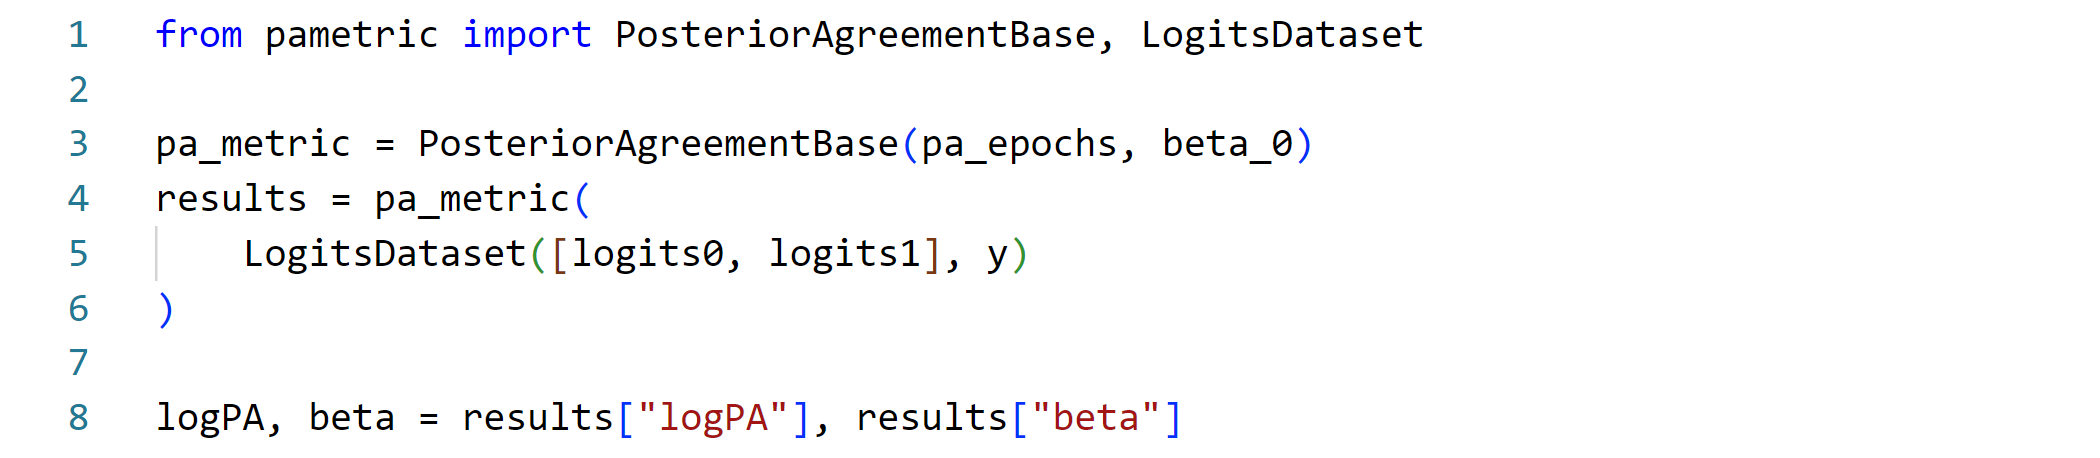
\includegraphics[width=0.98\textwidth]{img/theoretical_background/pametric_code.png}  % Your image here
    % }
}

\begin{properties}[PA metric implementation]
    The most relevant features of the numerical implementation of the metric are the following:
\begin{itemize}
    \item The metric launches a single optimization process with a pair of datasets. Nevertheless, 
    additional datasets can be added for validation purposes. The metric also accepts different models,
    which can be useful in cross-validation settings.
    \item If data samples are not corresponding between datasets, the metric can implement several
    pairing strategies, namely label matching, nearest-neighbor or canonical correlation.
    \item Multi-device computation is supported. In particular, a distributed-data-processing (DDP)
    strategy on a CUDA-managed set of GPUs can be used to parallelize model evaluation.
    \item The output of the model is computed just once per training epoch, which reduces drastically
    the time required for the optimization of the kernel.
    \item Detailed information about the optimization process can be easily retrieved and logged, which helps
    tuning the optimization algorithm and other hyperparameters.
\end{itemize}
\end{properties}

The complete code implementation along with the set of unit tests conducted 
to ensure consistency between training and data processing strategies can be 
found in the \texttt{pa-metric} repository\footnote{https://github.com/viictorjimenezzz/pa-metric}.

